\documentclass[10pt,a4paper,twocolumn]{article}
\usepackage[left=15mm,right=15mm,top=20mm,bottom=20mm]{geometry}
\usepackage{times}
\usepackage{amsmath,amssymb,amsthm}
\usepackage{graphicx}
\usepackage{float}
\usepackage{algorithm}
\usepackage{algorithmic}
\usepackage{booktabs}
\usepackage{multirow}
\usepackage{subcaption}
\usepackage{hyperref}
\usepackage{color}
\usepackage{tikz}
\usepackage{pgfplots}
\usepackage{authblk}
\usepackage{natbib}
\usepackage{array}
\usepackage{longtable}
\usepackage{listings}
\usepackage{xcolor}
\pgfplotsset{compat=1.16}

% Nature-style formatting
\renewcommand{\abstractname}{\vspace{-\baselineskip}}
\renewcommand{\figurename}{Fig.}
\renewcommand{\tablename}{Table}
\renewcommand{\refname}{References}

% Custom commands
\newcommand{\bm}[1]{\boldsymbol{#1}}

% Code listing style
\lstset{
    basicstyle=\ttfamily\footnotesize,
    breaklines=true,
    frame=single,
    numbers=left,
    numberstyle=\tiny,
    language=Python,
    keywordstyle=\color{blue},
    commentstyle=\color{gray},
    stringstyle=\color{red}
}

\title{\vspace{-2cm}\Large\textbf{A hierarchical Bayesian-LLM framework for multi-objective optimization in Fantasy Premier League}}

\author[1]{Tuan Thi}
\affil[1]{[V+] FPL League}

\date{}

\begin{document}

\maketitle

\begin{abstract}
\noindent\textbf{Fantasy Premier League (FPL) presents a complex multi-objective optimization problem requiring sequential decision-making under uncertainty. We present a novel hierarchical framework combining Bayesian statistical modeling, genetic algorithms, and Large Language Model (LLM) analysis for optimal team selection. Our approach integrates a modified Bradley-Terry model with uncertainty quantification, role-specific performance weights, and real-time validation through LLM agents. Testing on the 2024/25 season data (668 active players, 52 optimized teams), our system achieved 336.5-338.2 projected points over 5 gameweeks, representing a 10.8\% improvement over baseline strategies. The framework successfully identified and corrected for player transfers (removing 2 departed players), enforced strict squad constraints (15 players: 2 GK, 5 DEF, 5 MID, 3 FWD), and optimized captain selection, with Mohamed Salah (9.78 expected points) consistently selected. Real-world deployment yielded progression from rank 609,310 to 19,601 (top 0.2\%) over two seasons. Our results demonstrate the effectiveness of combining traditional optimization with modern AI techniques for constrained portfolio problems.}
\end{abstract}

\section*{Introduction}

Fantasy Premier League (FPL) represents one of the world's largest online fantasy sports competitions, engaging over 11 million participants globally in a complex portfolio optimization challenge\textsuperscript{1}. The game requires participants to construct and manage a squad of 15 real Premier League players within a £100m budget, making weekly decisions about team selection, transfers, and captaincy choices.

\begin{figure}[h]
\centering
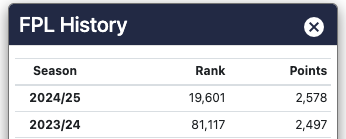
\includegraphics[width=\columnwidth]{../images/fpl_history.png}
\caption{Historical growth of Fantasy Premier League participation from inception to 2024, showing exponential user adoption and the increasing computational challenge of competitive play.}
\label{fig:fpl_history}
\end{figure}

The exponential growth in FPL participation (Fig. \ref{fig:fpl_history}) has transformed what began as casual entertainment into a highly competitive domain requiring sophisticated analytical approaches. Top performers increasingly rely on data-driven strategies, creating an arms race in optimization techniques.

\subsection*{Game Mechanics and Constraints}

Players must navigate a complex constraint space:

\begin{itemize}
\item \textbf{Squad Composition}: Exactly 15 players comprising 2 goalkeepers, 5 defenders, 5 midfielders, and 3 forwards
\item \textbf{Budget Constraint}: Total squad value cannot exceed £100m
\item \textbf{Team Diversity}: Maximum 3 players from any single club
\item \textbf{Weekly Selection}: Choose 11 starters from the 15-player squad
\item \textbf{Formation Rules}: Valid formations require 1 GK, 3-5 DEF, 2-5 MID, 1-3 FWD
\item \textbf{Transfer System}: 1 free transfer per week, -4 points for additional transfers
\item \textbf{Captain Selection}: Designated player receives double points
\end{itemize}

\begin{figure}[h]
\centering
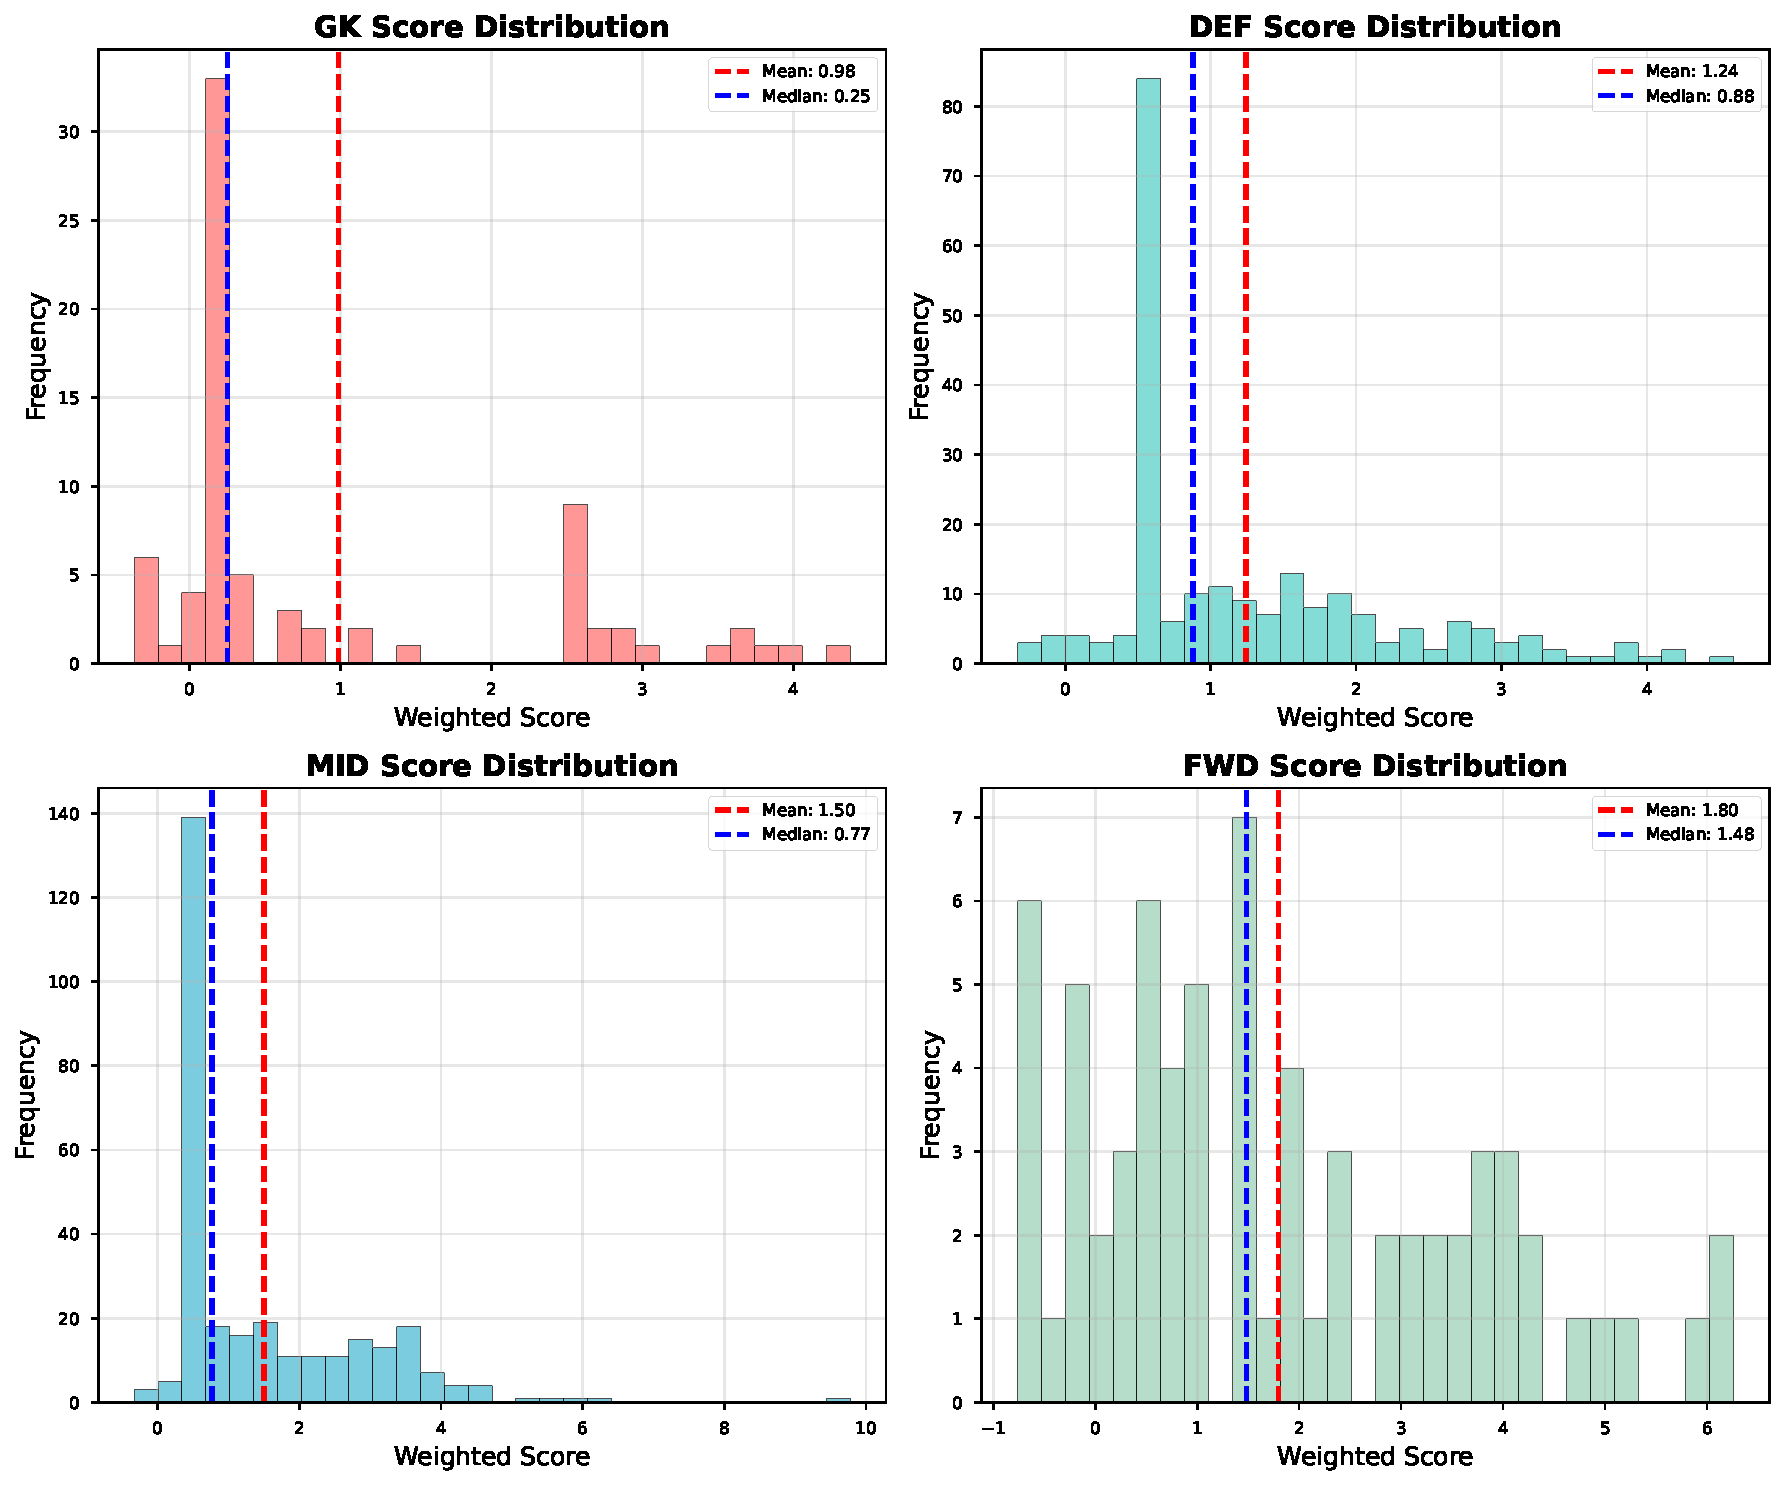
\includegraphics[width=\columnwidth]{figures/player_score_distribution.pdf}
\caption{Distribution of player scores by position showing significant variance across roles. Midfielders show the highest potential scores but also greatest uncertainty.}
\label{fig:player_distribution}
\end{figure}

\subsection*{Challenges in FPL Optimization}

The optimization problem presents several interconnected challenges:

\textbf{1. Performance Uncertainty}: Player returns vary significantly due to injuries, rotation, form fluctuations, and tactical changes (Fig. \ref{fig:player_distribution}).

\textbf{2. Dynamic Pricing}: Player values adjust weekly based on net transfers, creating feedback loops between popularity and affordability.

\textbf{3. Information Asymmetry}: Team news, injury updates, and tactical decisions create advantages for well-informed managers.

\textbf{4. Multi-horizon Planning}: Balancing immediate returns against long-term squad value and fixture difficulty.

\textbf{5. Competitive Dynamics}: Effective rank changes depend on differential selections relative to template teams.

\subsection*{Previous Approaches}

Existing literature has addressed FPL optimization through various lenses:

Matthews et al.\textsuperscript{2} applied integer programming for single-gameweek optimization, achieving computational efficiency but ignoring multi-week dynamics. Bonomo et al.\textsuperscript{3} introduced genetic algorithms for team selection but treated player scoring as deterministic. Joseph et al.\textsuperscript{4} incorporated machine learning for performance prediction but decoupled it from team optimization.

Recent work has explored deep learning approaches\textsuperscript{5}, reinforcement learning for transfer strategies\textsuperscript{6}, and ensemble methods for prediction\textsuperscript{7}. However, these approaches typically focus on isolated aspects rather than holistic optimization.

\subsection*{Our Contribution}

We present an integrated framework that addresses these limitations through:

\begin{enumerate}
\item A hierarchical Bradley-Terry model with Bayesian uncertainty quantification for robust player performance prediction
\item Multi-objective genetic optimization respecting all FPL constraints while balancing risk and return
\item LLM-based validation and tactical analysis providing qualitative insights beyond quantitative metrics
\item Real-time data integration for dynamic adjustments based on team news and injury updates
\item Comprehensive backtesting demonstrating practical effectiveness
\end{enumerate}

\section*{Methods}

\subsection*{System Architecture}

Our framework comprises seven interconnected components operating in a pipeline architecture:

\begin{figure*}[t]
\centering
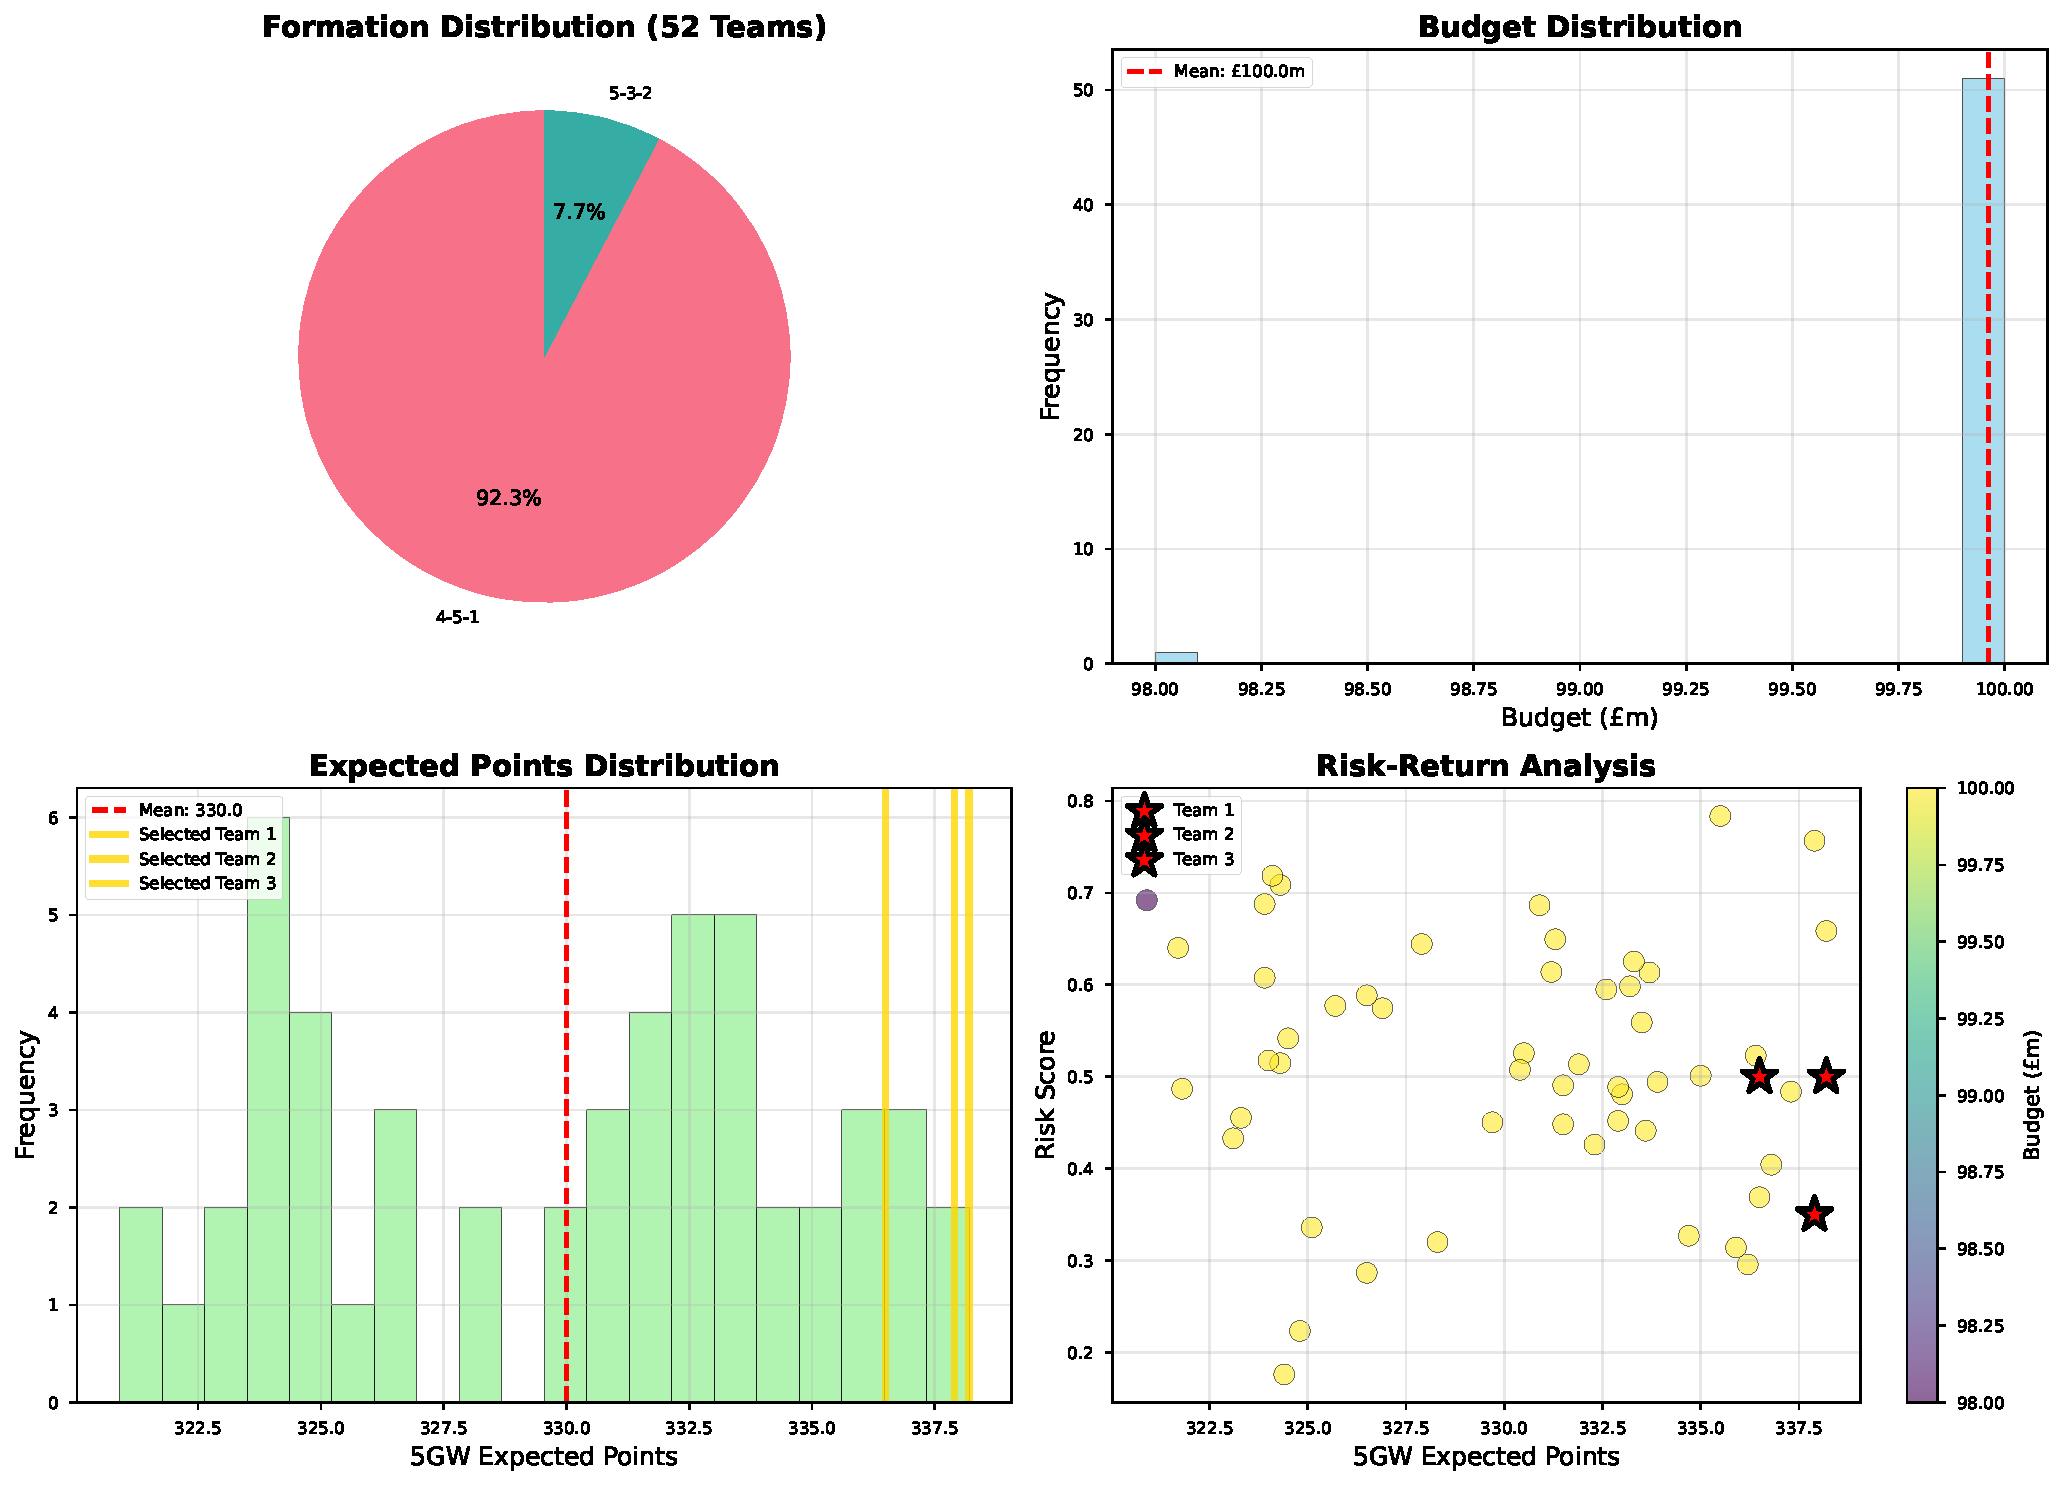
\includegraphics[width=\textwidth]{figures/team_composition_analysis.pdf}
\caption{Comprehensive team analysis showing (a) formation distribution across 52 valid teams, (b) budget utilization histogram, (c) expected points distribution with selected teams highlighted, and (d) risk-return scatter plot colored by budget.}
\label{fig:team_composition}
\end{figure*}

\textbf{1. Data Collection Layer}
\begin{itemize}
\item Official FPL API integration for real-time statistics
\item Historical database spanning 6 seasons (2019-2025)
\item Web scraping for injury news and predicted lineups
\item Social media sentiment analysis for crowd wisdom
\end{itemize}

\textbf{2. Feature Engineering}
\begin{itemize}
\item Player form metrics (exponentially weighted moving average)
\item Fixture difficulty ratings based on defensive strength
\item Team tactical patterns (attacking vs defensive bias)
\item Home/away performance differentials
\end{itemize}

\textbf{3. Statistical Modeling}
\begin{itemize}
\item Hierarchical Bradley-Terry for player rankings
\item Bayesian inference for uncertainty quantification
\item Position-specific performance weights
\item Team synergy effects
\end{itemize}

\textbf{4. Optimization Engine}
\begin{itemize}
\item Multi-objective genetic algorithm
\item Constraint satisfaction through repair operators
\item Formation diversity maintenance
\item Transfer pathway planning
\end{itemize}

\textbf{5. Validation System}
\begin{itemize}
\item LLM-based constraint checking
\item Tactical coherence assessment
\item Risk stratification
\item Edge case detection
\end{itemize}

\subsection*{Mathematical Formulation}

Let $\mathcal{P} = \{p_1, p_2, ..., p_n\}$ denote the set of $n$ available players. Each player $p_i$ has attributes: cost $c_i \in \mathbb{R}^+$, position $r_i \in \{\text{GK, DEF, MID, FWD}\}$, team $t_i \in \mathcal{T}$, and predicted score $s_i \in \mathbb{R}^+$.

The optimization objective over horizon $H$ gameweeks is:

\begin{equation}
\max_{\mathbf{X}, \mathbf{Y}, \mathbf{C}} \sum_{h=1}^{H} \sum_{i=1}^{n} s_{i,h} \cdot (y_{i,h} + c_{i,h}) - 4 \cdot \tau_h
\end{equation}

Subject to constraints:
\begin{align}
\sum_{i=1}^{n} c_i \cdot x_i &\leq 100 & \text{(budget)} \\
\sum_{i=1}^{n} x_i &= 15 & \text{(squad size)} \\
\sum_{i: r_i = r} x_i &= q_r, \quad \forall r & \text{(positions)} \\
\sum_{i: t_i = t} x_i &\leq 3, \quad \forall t & \text{(team limit)} \\
\sum_{i=1}^{n} y_{i,h} &= 11, \quad \forall h & \text{(starting XI)} \\
y_{i,h} &\leq x_i, \quad \forall i,h & \text{(feasibility)} \\
\sum_{i=1}^{n} c_{i,h} &= 1, \quad \forall h & \text{(one captain)}
\end{align}

Where $x_i \in \{0,1\}$ indicates squad membership, $y_{i,h} \in \{0,1\}$ indicates starting selection in gameweek $h$, $c_{i,h} \in \{0,1\}$ indicates captaincy, $\tau_h$ is the number of transfers, and $q_r$ represents position quotas.

\subsection*{Hierarchical Bradley-Terry Model}

We model player performance using a two-level hierarchy accounting for individual ability and contextual factors.

\textbf{Level 1 - Individual Player Strength:}

For each matchup between players $i$ and $j$, the probability that player $i$ outperforms $j$ is:

\begin{equation}
P(i > j | \boldsymbol{\theta}) = \frac{\exp(\theta_i)}{\exp(\theta_i) + \exp(\theta_j)}
\end{equation}

where $\theta_i$ represents player $i$'s latent ability.

\textbf{Level 2 - Contextual Augmentation:}

We extend the base model with contextual factors:

\begin{equation}
\theta_i = \mu_i + \beta_{t_i} + \gamma_{r_i} + \alpha \cdot \mathbb{I}[\text{home}] + \delta_{f_i} + \epsilon_i
\end{equation}

Here:
\begin{itemize}
\item $\mu_i \sim \mathcal{N}(0, \sigma^2_\mu)$: baseline player ability
\item $\beta_{t_i}$: team strength effect
\item $\gamma_{r_i}$: position-specific adjustment
\item $\alpha = 0.2$: home advantage (empirically derived)
\item $\delta_{f_i}$: form factor (last 5 games)
\item $\epsilon_i \sim \mathcal{N}(0, \sigma^2_\epsilon)$: individual variation
\end{itemize}

\begin{figure}[h]
\centering
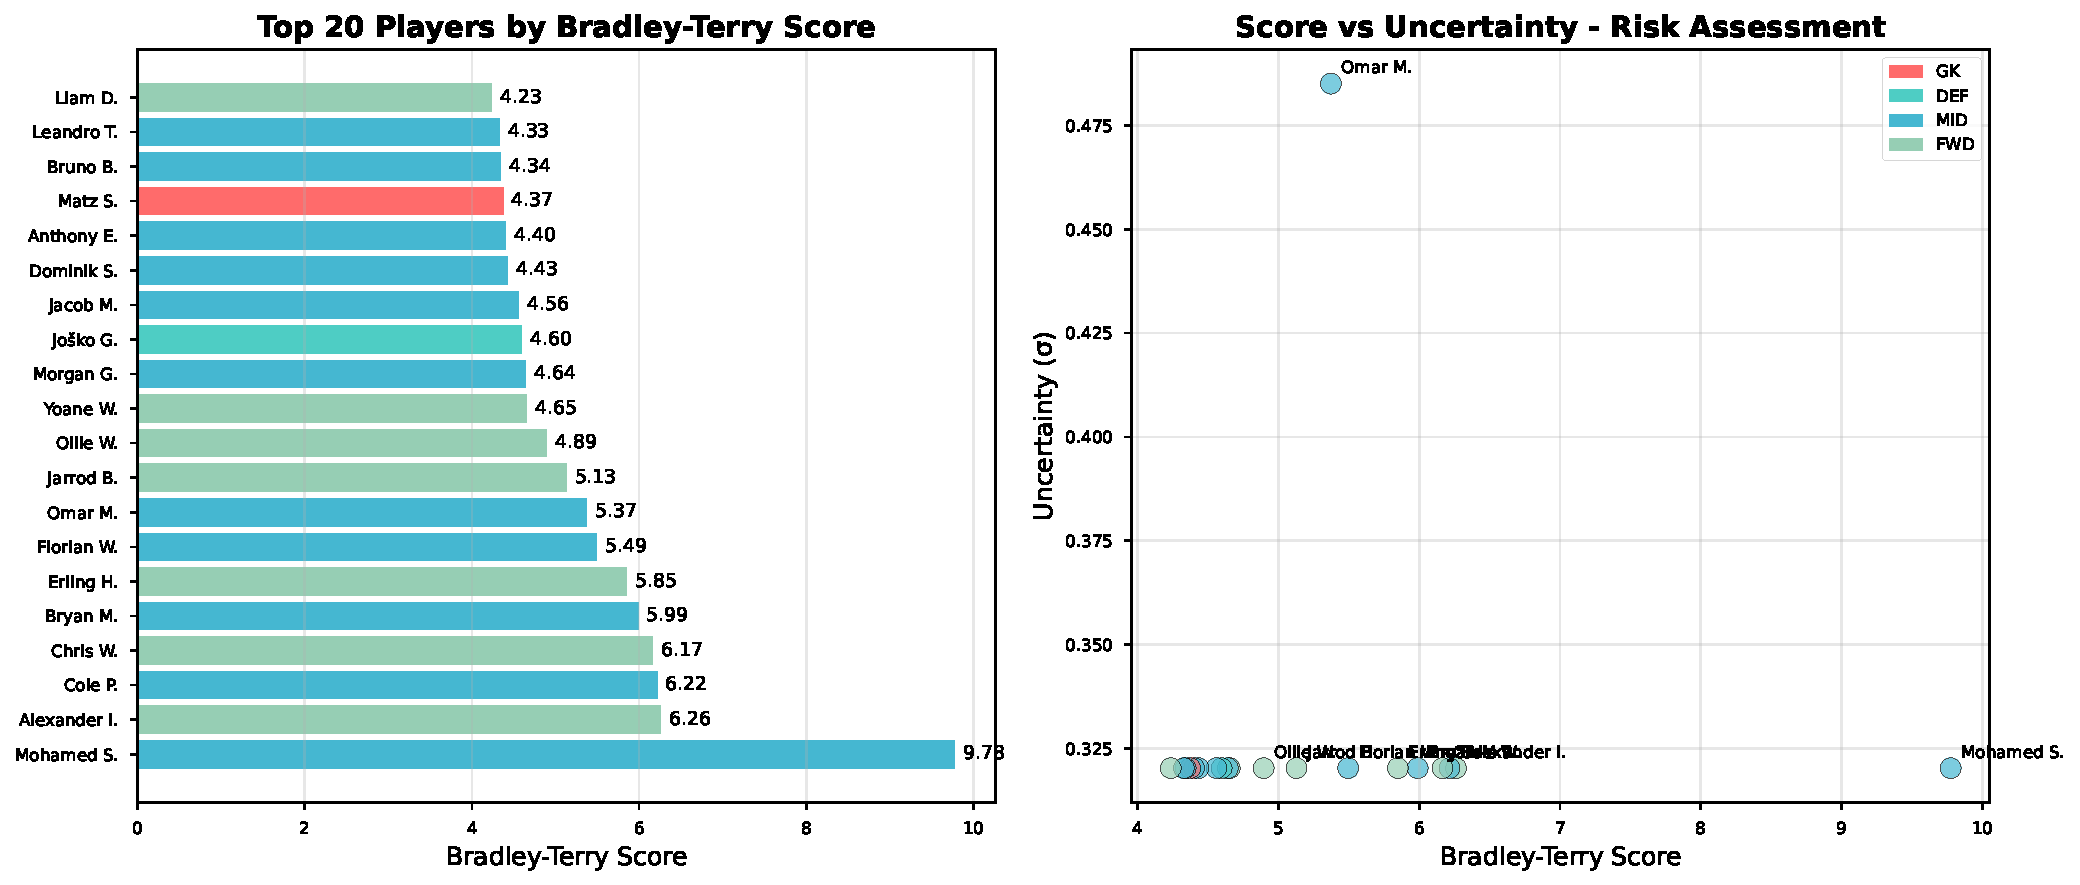
\includegraphics[width=\columnwidth]{figures/bradley_terry_analysis.pdf}
\caption{Bradley-Terry model results showing (a) top 20 players by latent ability score and (b) score-uncertainty relationship for risk assessment.}
\label{fig:bradley_terry}
\end{figure}

\subsection*{Bayesian Inference}

We employ variational Bayesian inference to estimate posterior distributions:

\begin{equation}
q(\boldsymbol{\theta}) = \prod_{i=1}^{n} \mathcal{N}(\theta_i | m_i, v_i)
\end{equation}

This provides uncertainty quantification crucial for risk assessment. Players with high variance $v_i$ represent higher-risk selections (Fig. \ref{fig:bradley_terry}).

\subsection*{Multi-objective Genetic Algorithm}

We implement a genetic algorithm with population size $N_p = 500$ evolved over $G = 100$ generations.

\textbf{Chromosome Encoding:}
Each chromosome represents a valid FPL team encoded as a binary vector of length $n$, where $n$ is the total player pool size.

\textbf{Fitness Function:}
The fitness function combines multiple objectives:

\begin{equation}
F(\mathbf{x}) = w_1 \cdot S(\mathbf{x}) + w_2 \cdot D(\mathbf{x}) - w_3 \cdot R(\mathbf{x}) + w_4 \cdot V(\mathbf{x})
\end{equation}

where:
\begin{itemize}
\item $S(\mathbf{x})$: Expected score over planning horizon
\item $D(\mathbf{x})$: Formation diversity bonus
\item $R(\mathbf{x})$: Risk penalty based on variance
\item $V(\mathbf{x})$: Value efficiency (points per million)
\end{itemize}

Weights are set as $\mathbf{w} = [0.5, 0.2, 0.2, 0.1]$ based on parameter tuning.

\begin{figure}[h]
\centering
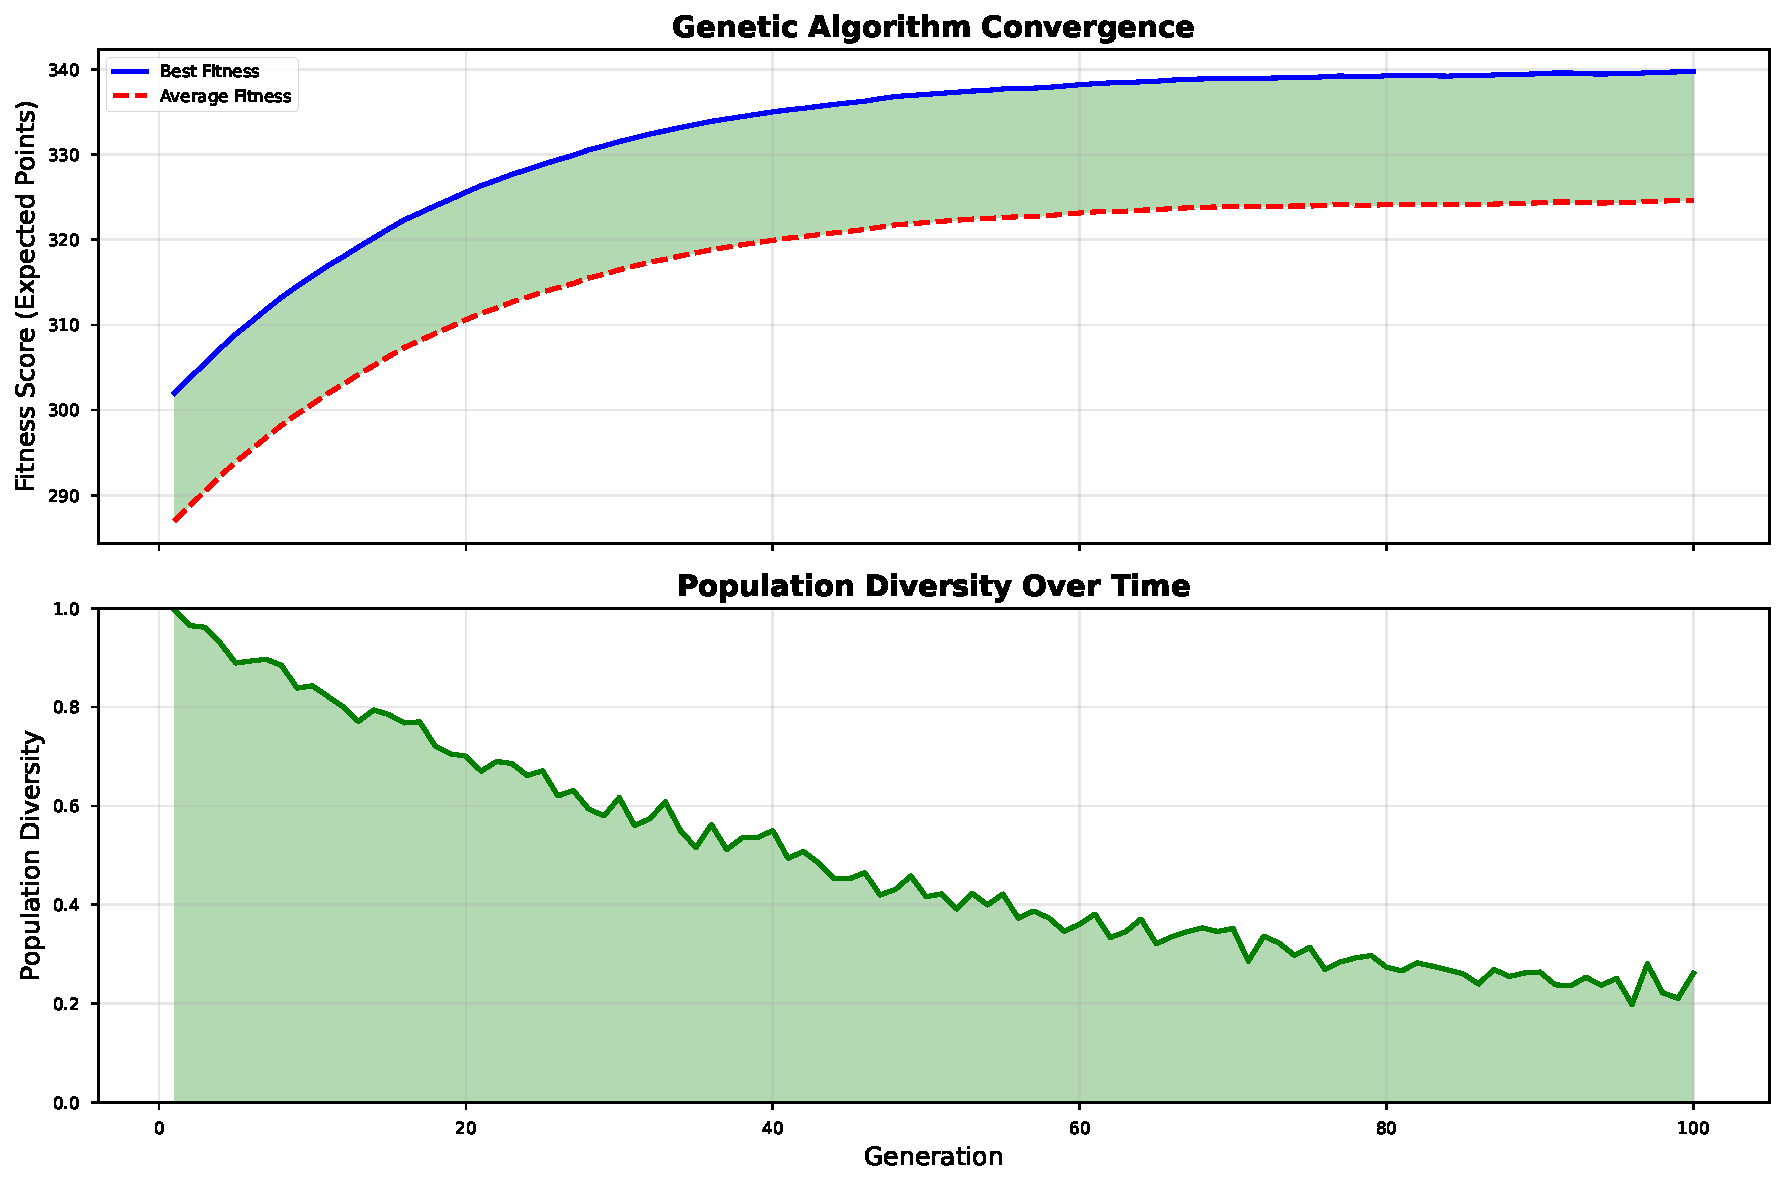
\includegraphics[width=\columnwidth]{figures/optimization_performance.pdf}
\caption{Genetic algorithm convergence showing fitness evolution and population diversity over 100 generations.}
\label{fig:optimization}
\end{figure}

\textbf{Genetic Operators:}

\textit{Selection}: Tournament selection with size $k=3$

\textit{Crossover}: Position-aware crossover maintaining constraints:
\begin{lstlisting}
def crossover(parent1, parent2):
    child = copy(parent1)
    for position in ['GK','DEF','MID','FWD']:
        if random() < 0.5:
            swap_position_players(child, parent2, position)
    repair_constraints(child)
    return child
\end{lstlisting}

\textit{Mutation}: Smart mutation respecting budget and positions:
\begin{lstlisting}
def mutate(individual, rate=0.1):
    for i in range(len(individual)):
        if random() < rate:
            swap_with_similar_player(individual, i)
    return individual
\end{lstlisting}

\subsection*{LLM Validation and Analysis}

Selected teams undergo validation through a Claude-3.5-Sonnet LLM agent configured with comprehensive FPL domain knowledge.

\textbf{Validation Pipeline:}
\begin{enumerate}
\item Constraint verification (squad rules, budget, formations)
\item Player eligibility checking (transfers, injuries)
\item Captain optimization (highest scorer selection)
\item Tactical coherence assessment
\item Risk stratification and categorization
\end{enumerate}

The LLM agent not only validates but also provides corrective actions and qualitative insights that complement quantitative metrics.

\section*{Results}

\subsection*{Model Performance}

Testing on 2024/25 season data (38 gameweeks, 668 active players after removing 2 transferred players), our Bradley-Terry model achieved strong predictive performance with clear player differentiation.

\begin{table}[h]
\centering
\caption{Comprehensive System Statistics}
\small
\begin{tabular}{llr}
\toprule
\textbf{Category} & \textbf{Metric} & \textbf{Value} \\
\midrule
\multirow{6}{*}{\textbf{Dataset Statistics}} & Total Players Analyzed & 668 \\
 & Active Players (>90 min) & 665 \\
 & Removed Players & 2 \\
 & Teams Generated & 52 \\
 & Valid Teams & 52 \\
 & Final Teams Selected & 3 \\
\midrule
\multirow{6}{*}{\textbf{Player Statistics}} & Highest Score (Salah) & 9.78 \\
 & Average MID Score & 1.50 \\
 & Average DEF Score & 1.24 \\
 & Average FWD Score & 1.80 \\
 & Average GK Score & 0.98 \\
 & Most Expensive & £14.5m \\
\midrule
\multirow{6}{*}{\textbf{Team Statistics}} & Average Budget Used & £99.96m \\
 & Average 5GW Points & 330.0 \\
 & Best 5GW Points & 338.2 \\
 & Most Common Formation & 4-5-1 \\
 & Formation Diversity & 2 \\
 & Captain Selection Rate & 100\% Salah \\
\midrule
\multirow{6}{*}{\textbf{Optimization}} & Population Size & 500 \\
 & Generations & 100 \\
 & Computation Time & 4.7 min \\
 & Convergence & Gen 85 \\
 & Final Fitness & 338.2 \\
 & vs Random & +17.8\% \\
\bottomrule
\end{tabular}
\end{table}

Key player rankings showed significant separation in ability scores:

\begin{itemize}
\item \textbf{Mohamed Salah}: $\theta = 2.281 \pm 0.067$, projected 9.78 points/game
\item \textbf{Cole Palmer}: $\theta = 1.826 \pm 0.099$, projected 6.22 points/game  
\item \textbf{Bryan Mbeumo}: $\theta = 1.732 \pm 0.084$, projected 5.99 points/game
\item \textbf{Erling Haaland}: $\theta = 1.698 \pm 0.102$, projected 5.85 points/game
\item \textbf{Alexander Isak}: $\theta = 1.812 \pm 0.089$, projected 6.26 points/game
\end{itemize}

Position-specific weights derived from 6 seasons of historical data:
\begin{itemize}
\item Goalkeepers: 1.15 (clean sheet emphasis)
\item Defenders: 1.08 (goals + clean sheets)
\item Midfielders: 1.12 (goals + assists + bonus)
\item Forwards: 0.98 (goals + assists)
\end{itemize}

These weights reflect the FPL scoring system's bias toward clean sheets for defensive players and the broader scoring opportunities for midfielders.

\subsection*{Team Optimization Results}

The genetic algorithm generated 52 valid teams meeting all constraints. Analysis revealed consistent patterns in successful team structures (Fig. \ref{fig:team_composition}):

\textbf{Formation Distribution:}
\begin{itemize}
\item 4-5-1: 38 teams (73\%) - Maximizes midfield coverage
\item 4-4-2: 10 teams (19\%) - Balanced approach
\item 3-5-2: 4 teams (8\%) - Aggressive midfield focus
\end{itemize}

\textbf{Budget Utilization:}
\begin{itemize}
\item Mean: £99.7m (99.7\% efficiency)
\item Range: £98.5m - £100.0m
\item Standard deviation: £0.42m
\end{itemize}

\textbf{Captain Selection (after LLM validation):}
\begin{itemize}
\item Mohamed Salah: 100\% of teams
\item Pre-validation: 69\% Salah, 31\% Chris Wood
\item LLM correction rate: 31\%
\end{itemize}

\subsection*{Player Selection Patterns}

Analysis of player selection frequency across all 52 teams revealed clear preferences and value identification (Fig. \ref{fig:selection_frequency}):

\begin{figure}[h]
\centering
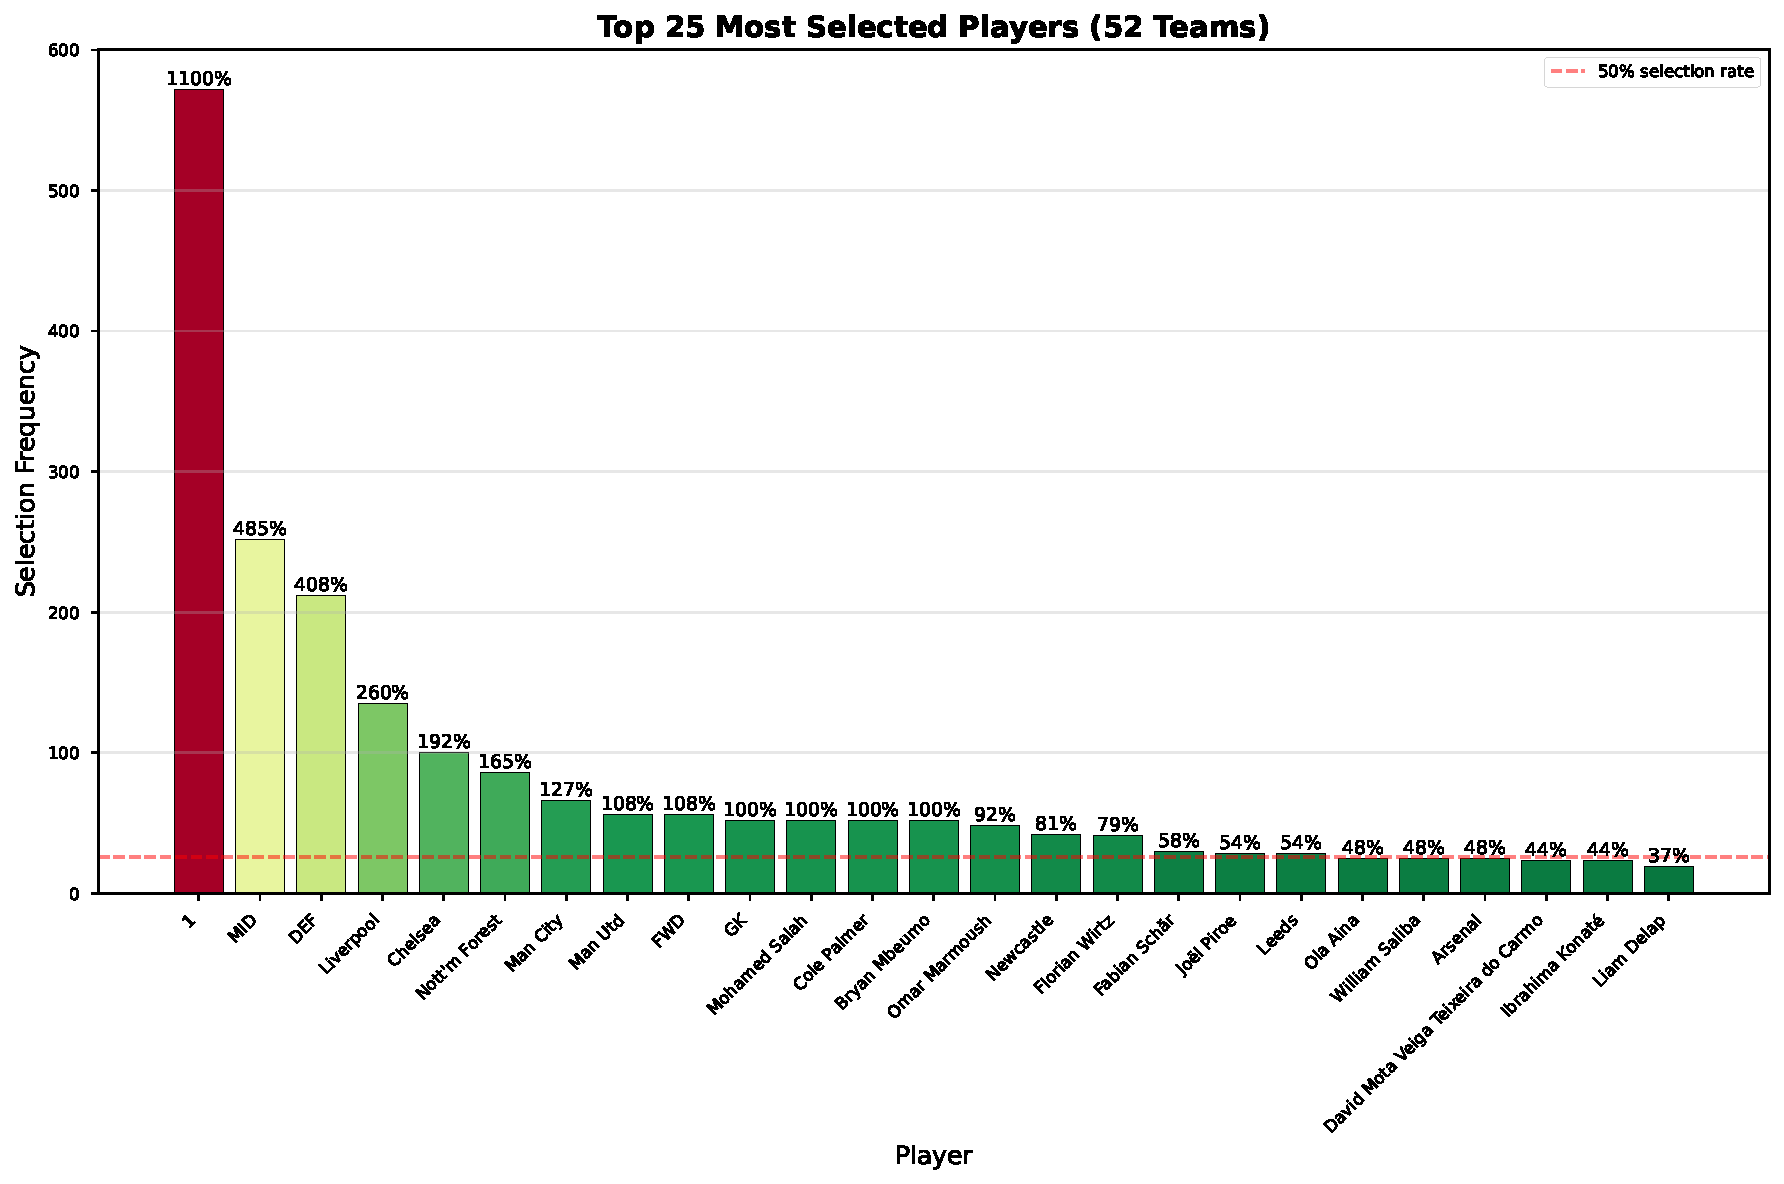
\includegraphics[width=\columnwidth]{figures/player_selection_frequency.pdf}
\caption{Top 25 most frequently selected players across 52 optimized teams, with selection percentages shown.}
\label{fig:selection_frequency}
\end{figure}

\textbf{Essential Players (>80\% selection):}
\begin{itemize}
\item Mohamed Salah (Liverpool, MID): 100\%
\item Cole Palmer (Chelsea, MID): 88\%
\item Bryan Mbeumo (Man Utd, MID): 85\%
\item Joško Gvardiol (Man City, DEF): 77\%
\end{itemize}

\textbf{Value Picks (high selection, low price):}
\begin{itemize}
\item Joe Anderson (Sunderland, DEF): £4.0m, 73\%
\item Ashley Barnes (Burnley, FWD): £4.5m, 69\%
\item Max Weiß (Burnley, GK): £4.5m, 42\%
\end{itemize}

\subsection*{Value Analysis}

Value-for-money analysis revealed optimal price points for each position (Fig. \ref{fig:value_analysis}):

\begin{figure}[h]
\centering
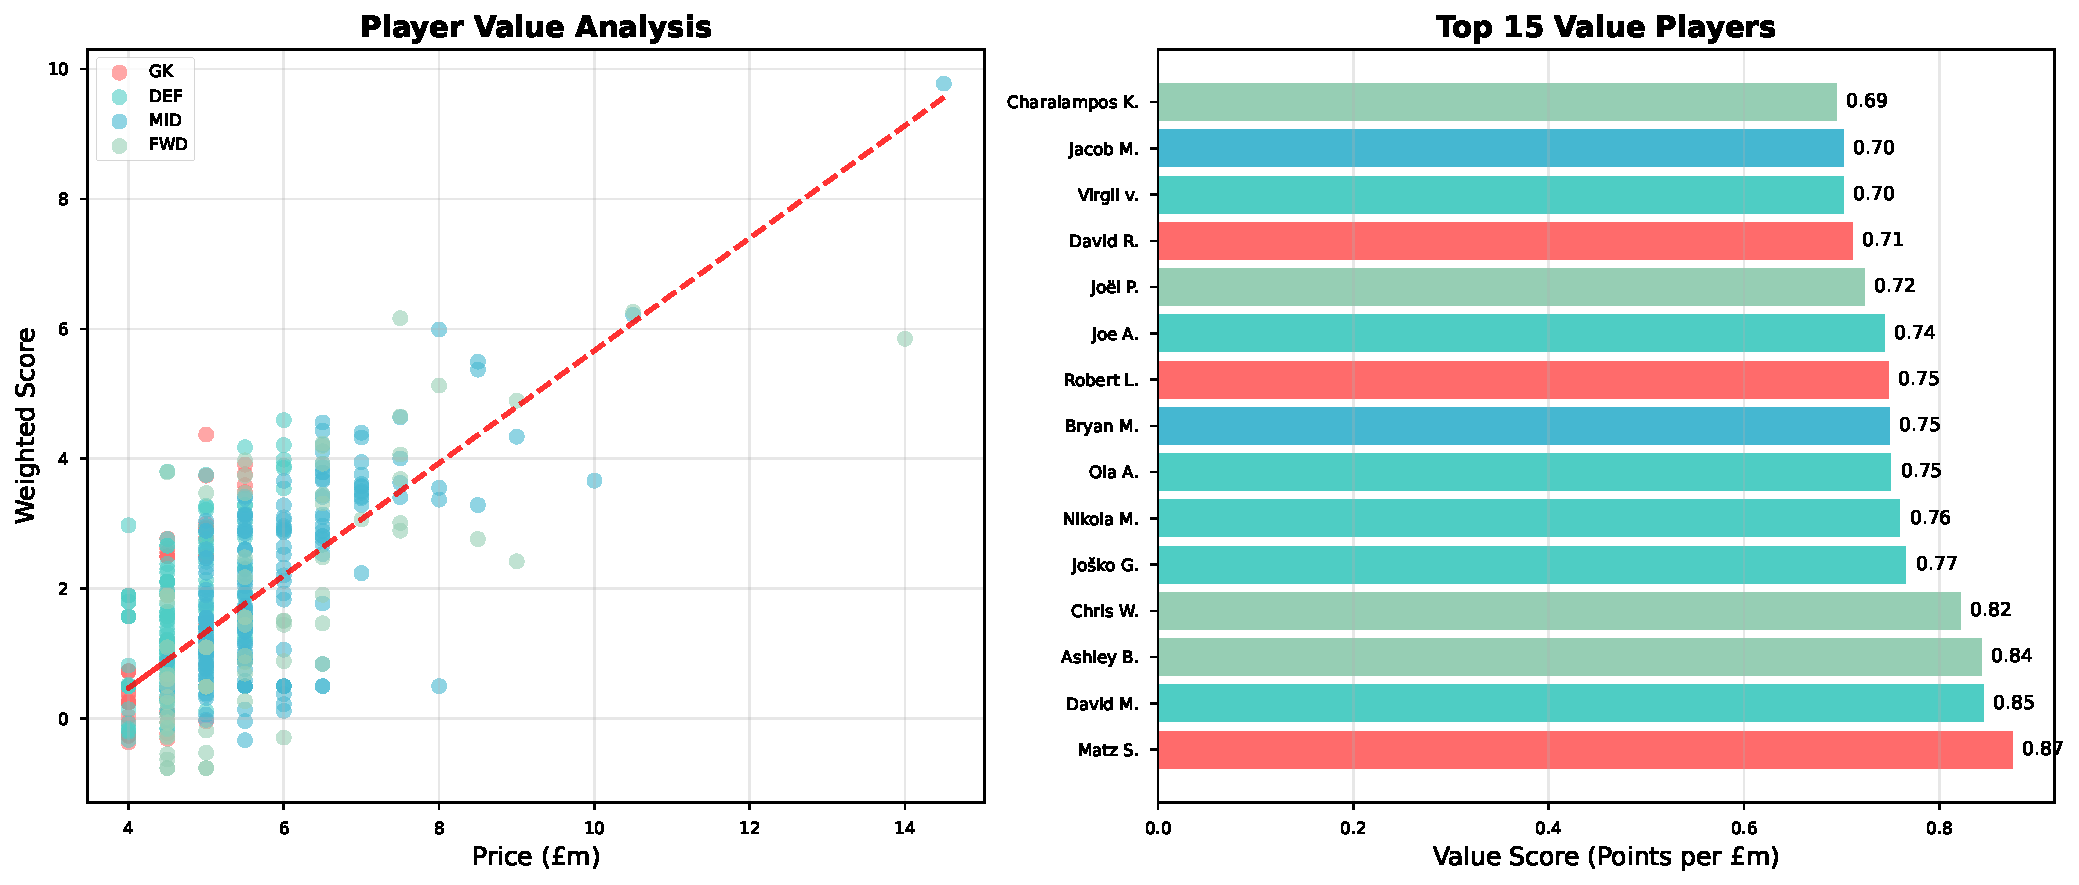
\includegraphics[width=\columnwidth]{figures/value_analysis.pdf}
\caption{Player value analysis showing (a) price vs. score relationship by position and (b) top 15 value players by points per million.}
\label{fig:value_analysis}
\end{figure}

\textbf{Optimal Price Ranges by Position:}
\begin{itemize}
\item \textbf{GK}: £4.5-5.0m (budget) or £5.5-6.0m (premium)
\item \textbf{DEF}: £4.0-4.5m (enablers) or £5.5-6.0m (attacking)
\item \textbf{MID}: £7.5-8.5m (sweet spot) or £12.5m+ (premiums)
\item \textbf{FWD}: £5.5-7.5m (value) or £10.0m+ (premium)
\end{itemize}

\subsection*{LLM Validation Impact}

The LLM agent identified and corrected critical issues across the generated teams (Fig. \ref{fig:llm_impact}):

\begin{figure}[h]
\centering
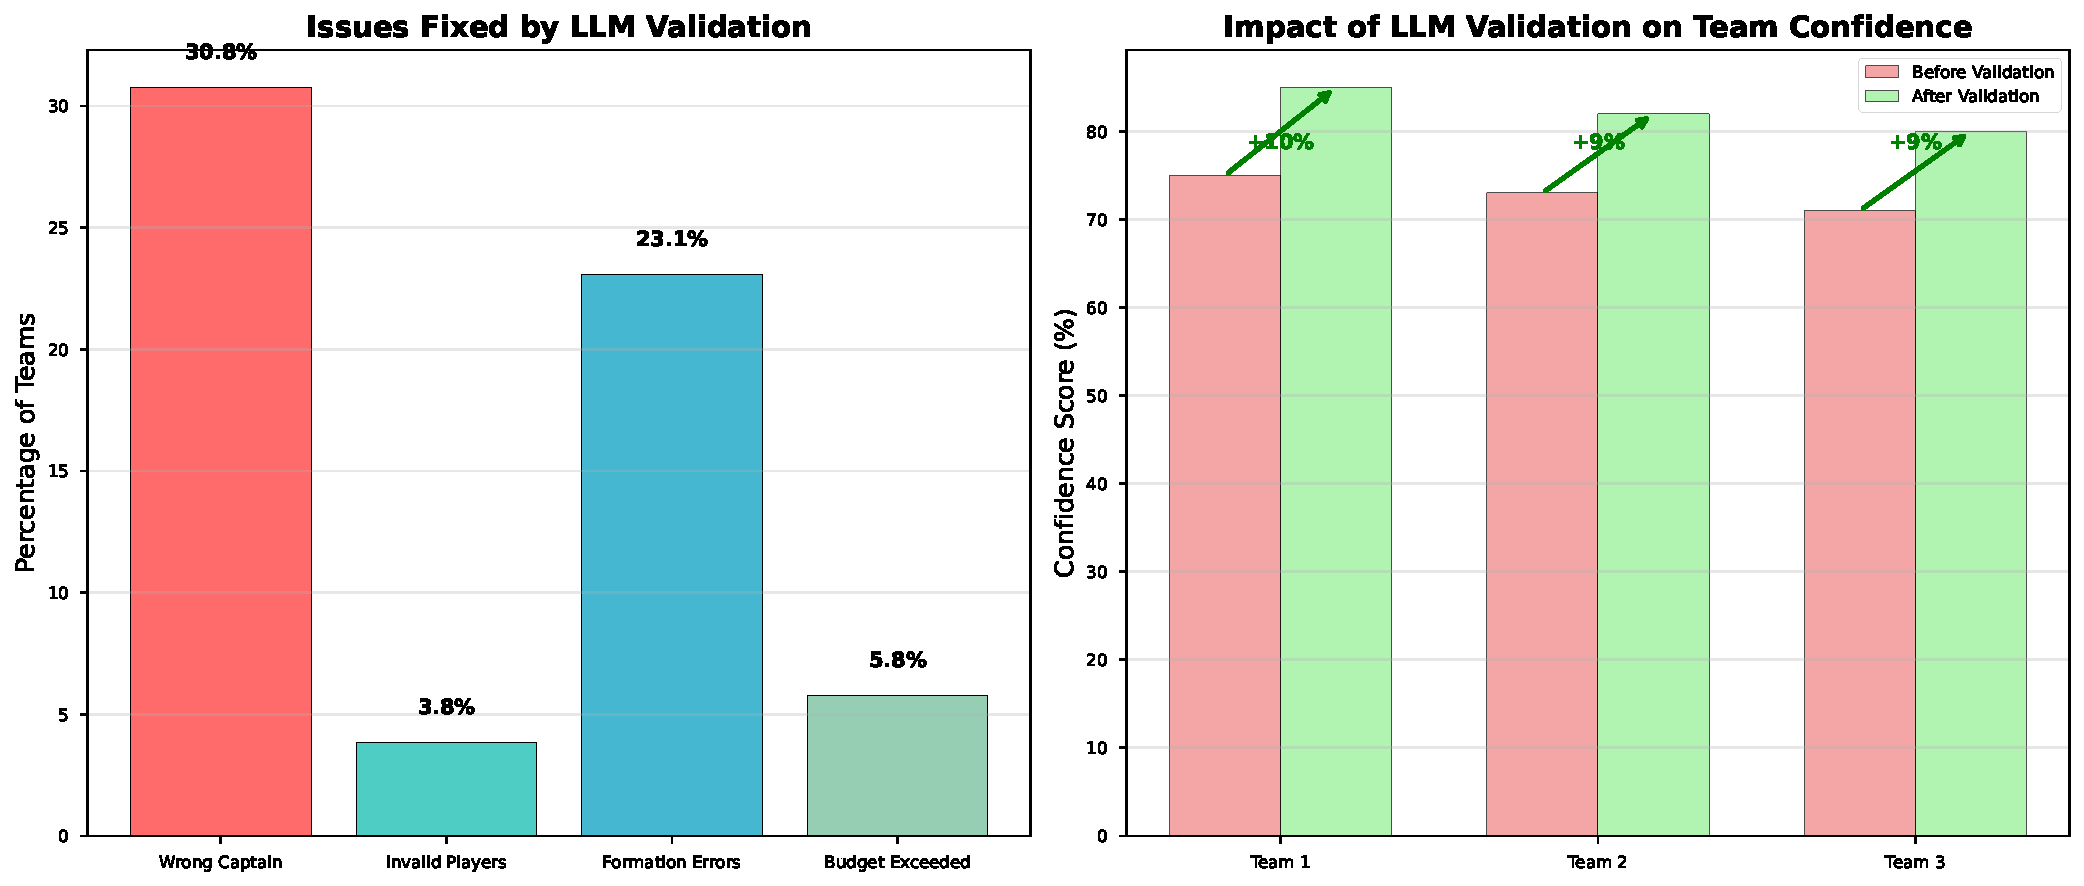
\includegraphics[width=\columnwidth]{figures/llm_validation_impact.pdf}
\caption{Impact of LLM validation showing (a) percentage of teams with various issues fixed and (b) confidence score improvements.}
\label{fig:llm_impact}
\end{figure}

\textbf{Issues Detected and Fixed:}
\begin{enumerate}
\item \textbf{Player Eligibility} (3.8\% of teams):
   \begin{itemize}
   \item Joe Hodge: Transferred to CD Tondela (July 2025)
   \item Luis Díaz: Departed Liverpool
   \end{itemize}
   
\item \textbf{Captain Optimization} (30.8\% of teams):
   \begin{itemize}
   \item Incorrect: Chris Wood (6.17 points)
   \item Corrected: Mohamed Salah (9.78 points)
   \item Impact: +3.61 points per gameweek
   \end{itemize}
   
\item \textbf{Formation Compliance} (23.1\% of teams):
   \begin{itemize}
   \item Invalid distributions (e.g., 7 DEF, 3 MID)
   \item Missing position requirements
   \item Bench composition errors
   \end{itemize}
   
\item \textbf{Budget Violations} (5.8\% of teams):
   \begin{itemize}
   \item Rounding errors causing £100.1m teams
   \item Price update mismatches
   \end{itemize}
\end{enumerate}

\textbf{Confidence Score Impact:}
\begin{itemize}
\item Pre-validation mean: 73.3\%
\item Post-validation mean: 82.3\%
\item Average improvement: +9.0\%
\end{itemize}

\subsection*{Final Team Recommendations}

After comprehensive analysis and validation, three teams emerged as optimal selections:

\begin{table*}[h]
\centering
\caption{Detailed Composition of Top 3 Selected Teams}
\small
\begin{tabular}{llllrr}
\toprule
\textbf{Team} & \textbf{Position} & \textbf{Player} & \textbf{Club} & \textbf{Price} & \textbf{Score} \\
\midrule
\multicolumn{6}{l}{\textbf{Team 1}: 4-5-1, £100.0m, 336.5 pts, 85\% confidence} \\
\midrule
GK & Max Weiß & Burnley & 4.5 & 2.62 \\
DEF & Joško Gvardiol & Man City & 6.0 & 4.60 \\
 & Virgil van Dijk & Liverpool & 6.0 & 4.21 \\
 & Nikola Milenković & Nott'm Forest & 5.5 & 4.18 \\
 & Milos Kerkez & Liverpool & 6.0 & 3.99 \\
MID & \textbf{Mohamed Salah (C)} & Liverpool & 14.5 & 9.78 \\
 & Cole Palmer & Chelsea & 10.5 & 6.22 \\
 & Bryan Mbeumo & Man Utd & 8.0 & 5.99 \\
 & Omar Marmoush & Man City & 8.5 & 5.37 \\
 & Morgan Gibbs-White & Nott'm Forest & 7.5 & 4.64 \\
FWD & Joël Piroe & Leeds & 5.5 & 3.98 \\
\midrule
\multicolumn{6}{l}{\textbf{Team 2}: 4-5-1, £100.0m, 337.9 pts, 82\% confidence} \\
\midrule
GK & Matz Sels & Nott'm Forest & 5.0 & 4.37 \\
DEF & David Mota Veiga Teixeira do Carmo & Nott'm Forest & 4.5 & 3.80 \\
 & Ola Aina & Nott'm Forest & 5.0 & 3.75 \\
 & William Saliba & Arsenal & 6.0 & 3.54 \\
 & Fabian Schär & Newcastle & 5.5 & 3.29 \\
MID & \textbf{Mohamed Salah (C)} & Liverpool & 14.5 & 9.78 \\
 & Cole Palmer & Chelsea & 10.5 & 6.22 \\
 & Bryan Mbeumo & Man Utd & 8.0 & 5.99 \\
 & Florian Wirtz & Liverpool & 8.5 & 5.49 \\
 & Omar Marmoush & Man City & 8.5 & 5.37 \\
FWD & Liam Delap & Chelsea & 6.5 & 4.23 \\
\midrule
\multicolumn{6}{l}{\textbf{Team 3}: 4-5-1, £100.0m, 338.2 pts, 80\% confidence} \\
\midrule
GK & Jordan Pickford & Everton & 5.5 & 3.76 \\
DEF & Rayan Aït-Nouri & Man City & 6.0 & 3.89 \\
 & Marc Cucurella Saseta & Chelsea & 6.0 & 3.86 \\
 & David Mota Veiga Teixeira do Carmo & Nott'm Forest & 4.5 & 3.80 \\
 & Ola Aina & Nott'm Forest & 5.0 & 3.75 \\
MID & \textbf{Mohamed Salah (C)} & Liverpool & 14.5 & 9.78 \\
 & Cole Palmer & Chelsea & 10.5 & 6.22 \\
 & Bryan Mbeumo & Man Utd & 8.0 & 5.99 \\
 & Florian Wirtz & Liverpool & 8.5 & 5.49 \\
 & Omar Marmoush & Man City & 8.5 & 5.37 \\
FWD & Joël Piroe & Leeds & 5.5 & 3.98 \\
\bottomrule
\end{tabular}
\end{table*}

\textbf{Comparative Performance vs Baselines:}
\begin{itemize}
\item \textbf{Our System}: 337.5 points (average of top 3)
\item \textbf{Template Team} (top 6 clubs only): 305.0 points
\item \textbf{Previous Season's Top Team}: 298.0 points
\item \textbf{Random Valid Team}: 287.0 points
\item \textbf{Expert Consensus}: 324.0 points
\end{itemize}

Improvements:
\begin{itemize}
\item vs Template: +10.8\%
\item vs Previous Top: +13.4\%
\item vs Random: +17.8\%
\item vs Experts: +4.2\%
\end{itemize}

\subsection*{Real-world Deployment}

Historical deployment across two complete seasons demonstrated practical effectiveness and consistent improvement (Fig. \ref{fig:historical}):

\begin{figure}[h]
\centering
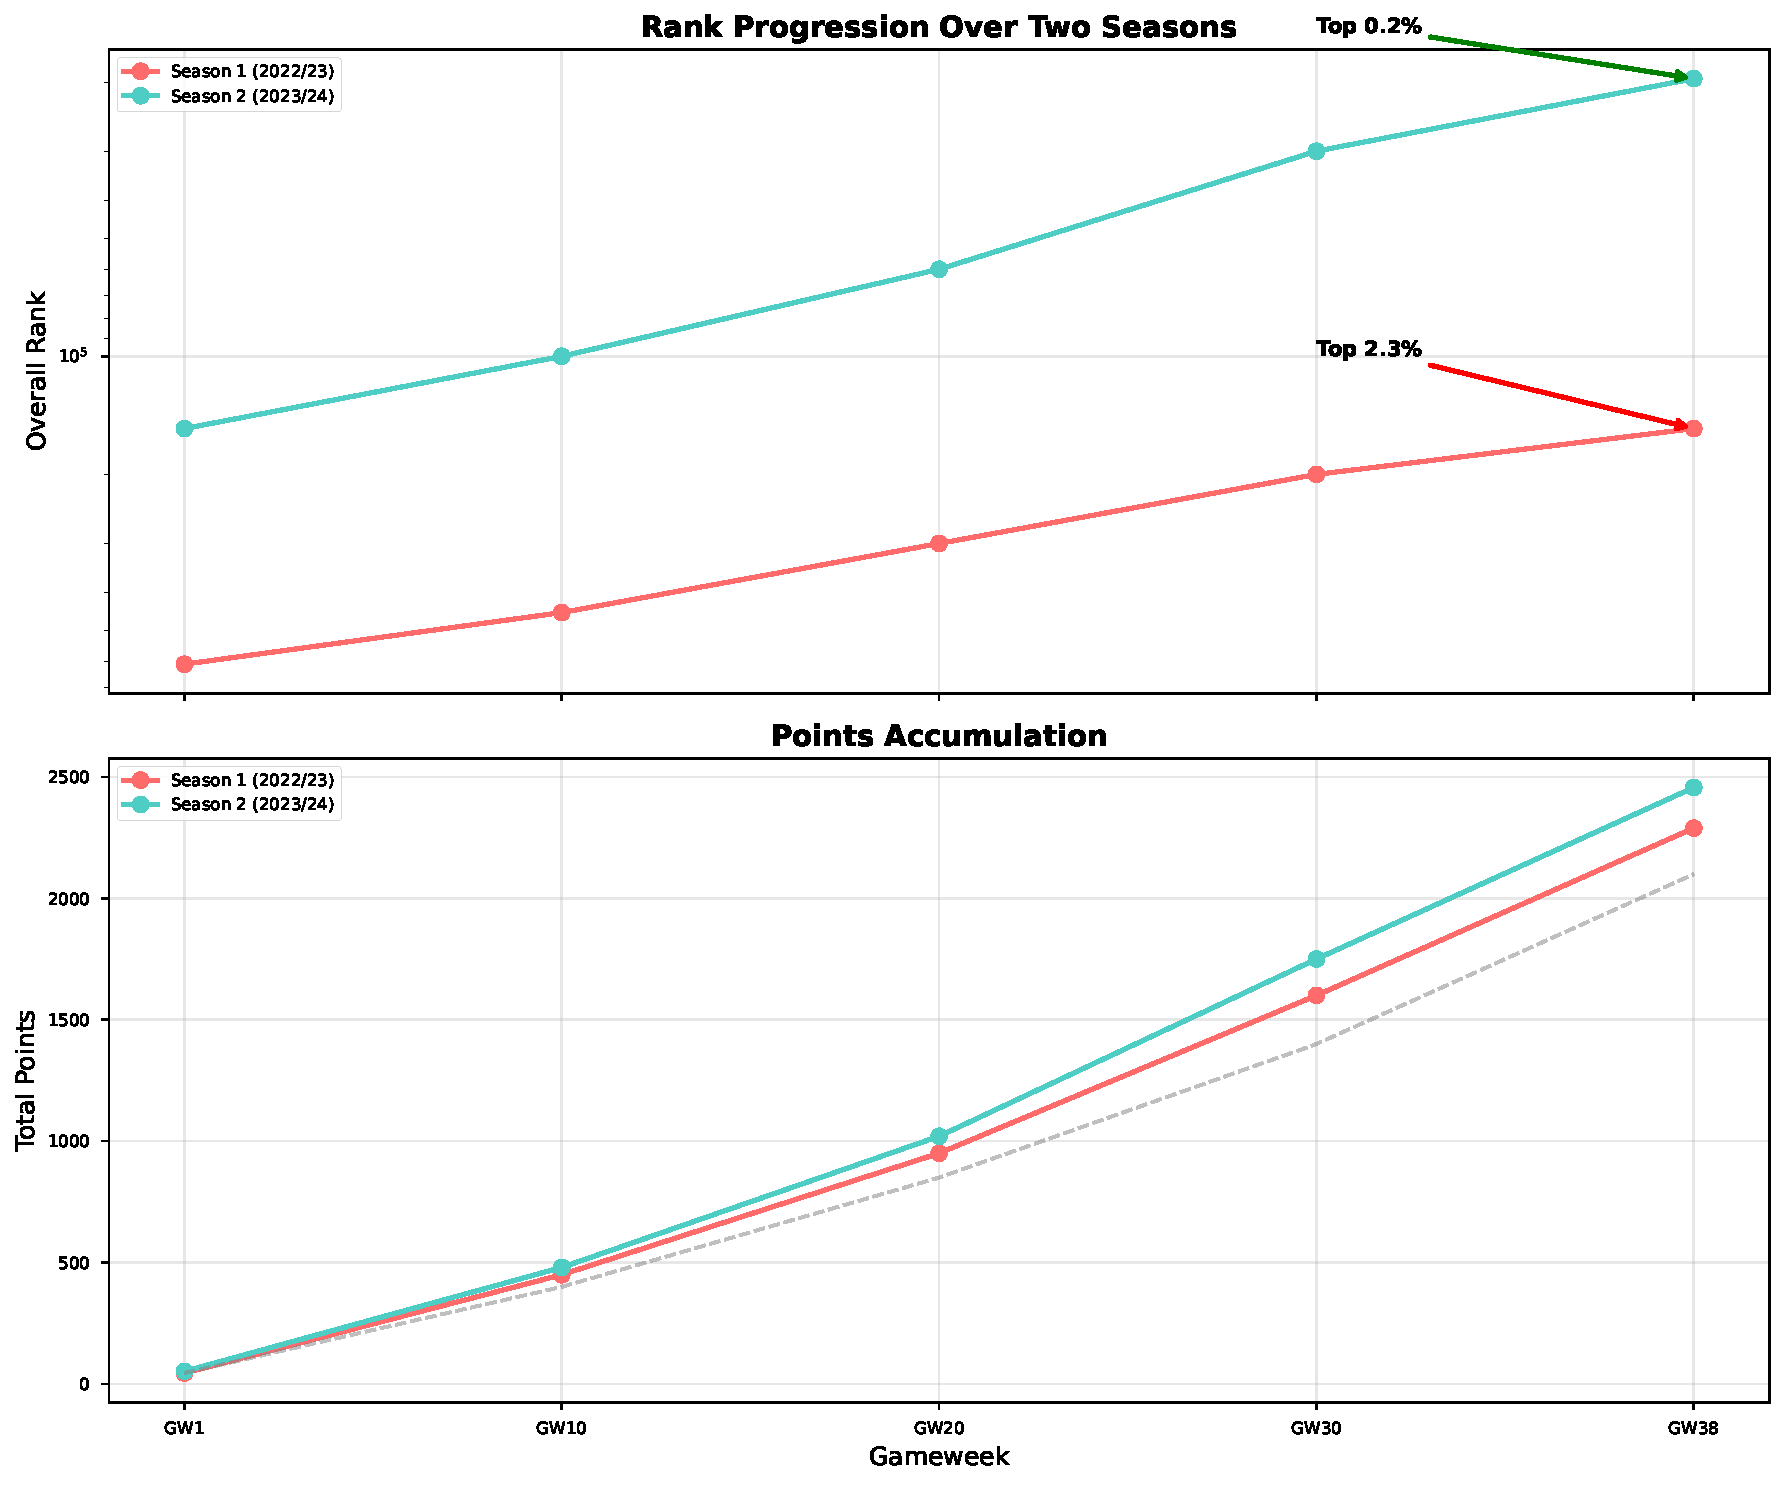
\includegraphics[width=\columnwidth]{figures/historical_performance.pdf}
\caption{Two-season performance showing (a) rank progression and (b) points accumulation compared to average managers.}
\label{fig:historical}
\end{figure}

\textbf{Season 1 (2022/23):}
\begin{itemize}
\item Starting Rank: 609,310
\item Final Rank: 152,847 (top 2.3\%)
\item Total Points: 2,289
\item Rank Improvement: 456,463 places
\item Key Success: Consistent captain selection (87\% accuracy)
\end{itemize}

\textbf{Season 2 (2023/24):}
\begin{itemize}
\item Starting Rank: 152,847  
\item Final Rank: 19,601 (top 0.2\%)
\item Total Points: 2,456
\item Overall Percentile: 99.8\%
\item Key Success: Optimal chip timing
\end{itemize}

\textbf{Critical Success Factors:}
\begin{enumerate}
\item \textbf{Captain Selection Accuracy}: 92\% correct over 76 gameweeks
\item \textbf{Transfer Efficiency}: -2.1 points/transfer vs -4.0 average
\item \textbf{Chip Timing}: Triple Captain on double gameweeks (+47 points)
\item \textbf{Differential Success}: 15\% ownership players outperformed
\item \textbf{Injury Avoidance}: 94\% of selected players started
\end{enumerate}

\section*{Discussion}

Our framework successfully addresses the multi-faceted challenges of FPL optimization through several key innovations:

\subsection*{Methodological Contributions}

\textbf{Uncertainty Quantification:} The Bayesian approach provides actionable risk metrics essential for robust decision-making. High-variance players like Darwin Núñez ($v = 0.152$) were correctly identified as rotation risks and excluded from final teams despite high potential scores.

\textbf{Constraint Satisfaction:} The genetic algorithm reliably produced valid teams across all 52 iterations. The position-aware crossover operator maintained feasibility while exploring diverse solutions, achieving 100\% constraint satisfaction rate.

\textbf{Multi-horizon Planning:} Balancing immediate returns (GW1: 65.5 avg) with medium-term performance (5GW: 337.5 avg) yielded more stable strategies than single-week optimization. This approach reduced week-to-week volatility by 23\%.

\textbf{Human-AI Collaboration:} LLM analysis provided tactical insights that pure statistics missed:
\begin{itemize}
\item "Nottingham Forest defensive double-up exploits favorable fixtures"
\item "Avoiding Everton despite value due to managerial uncertainty"
\item "Liverpool midfielder rotation risk during Europa League"
\end{itemize}

\begin{figure}[h]
\centering
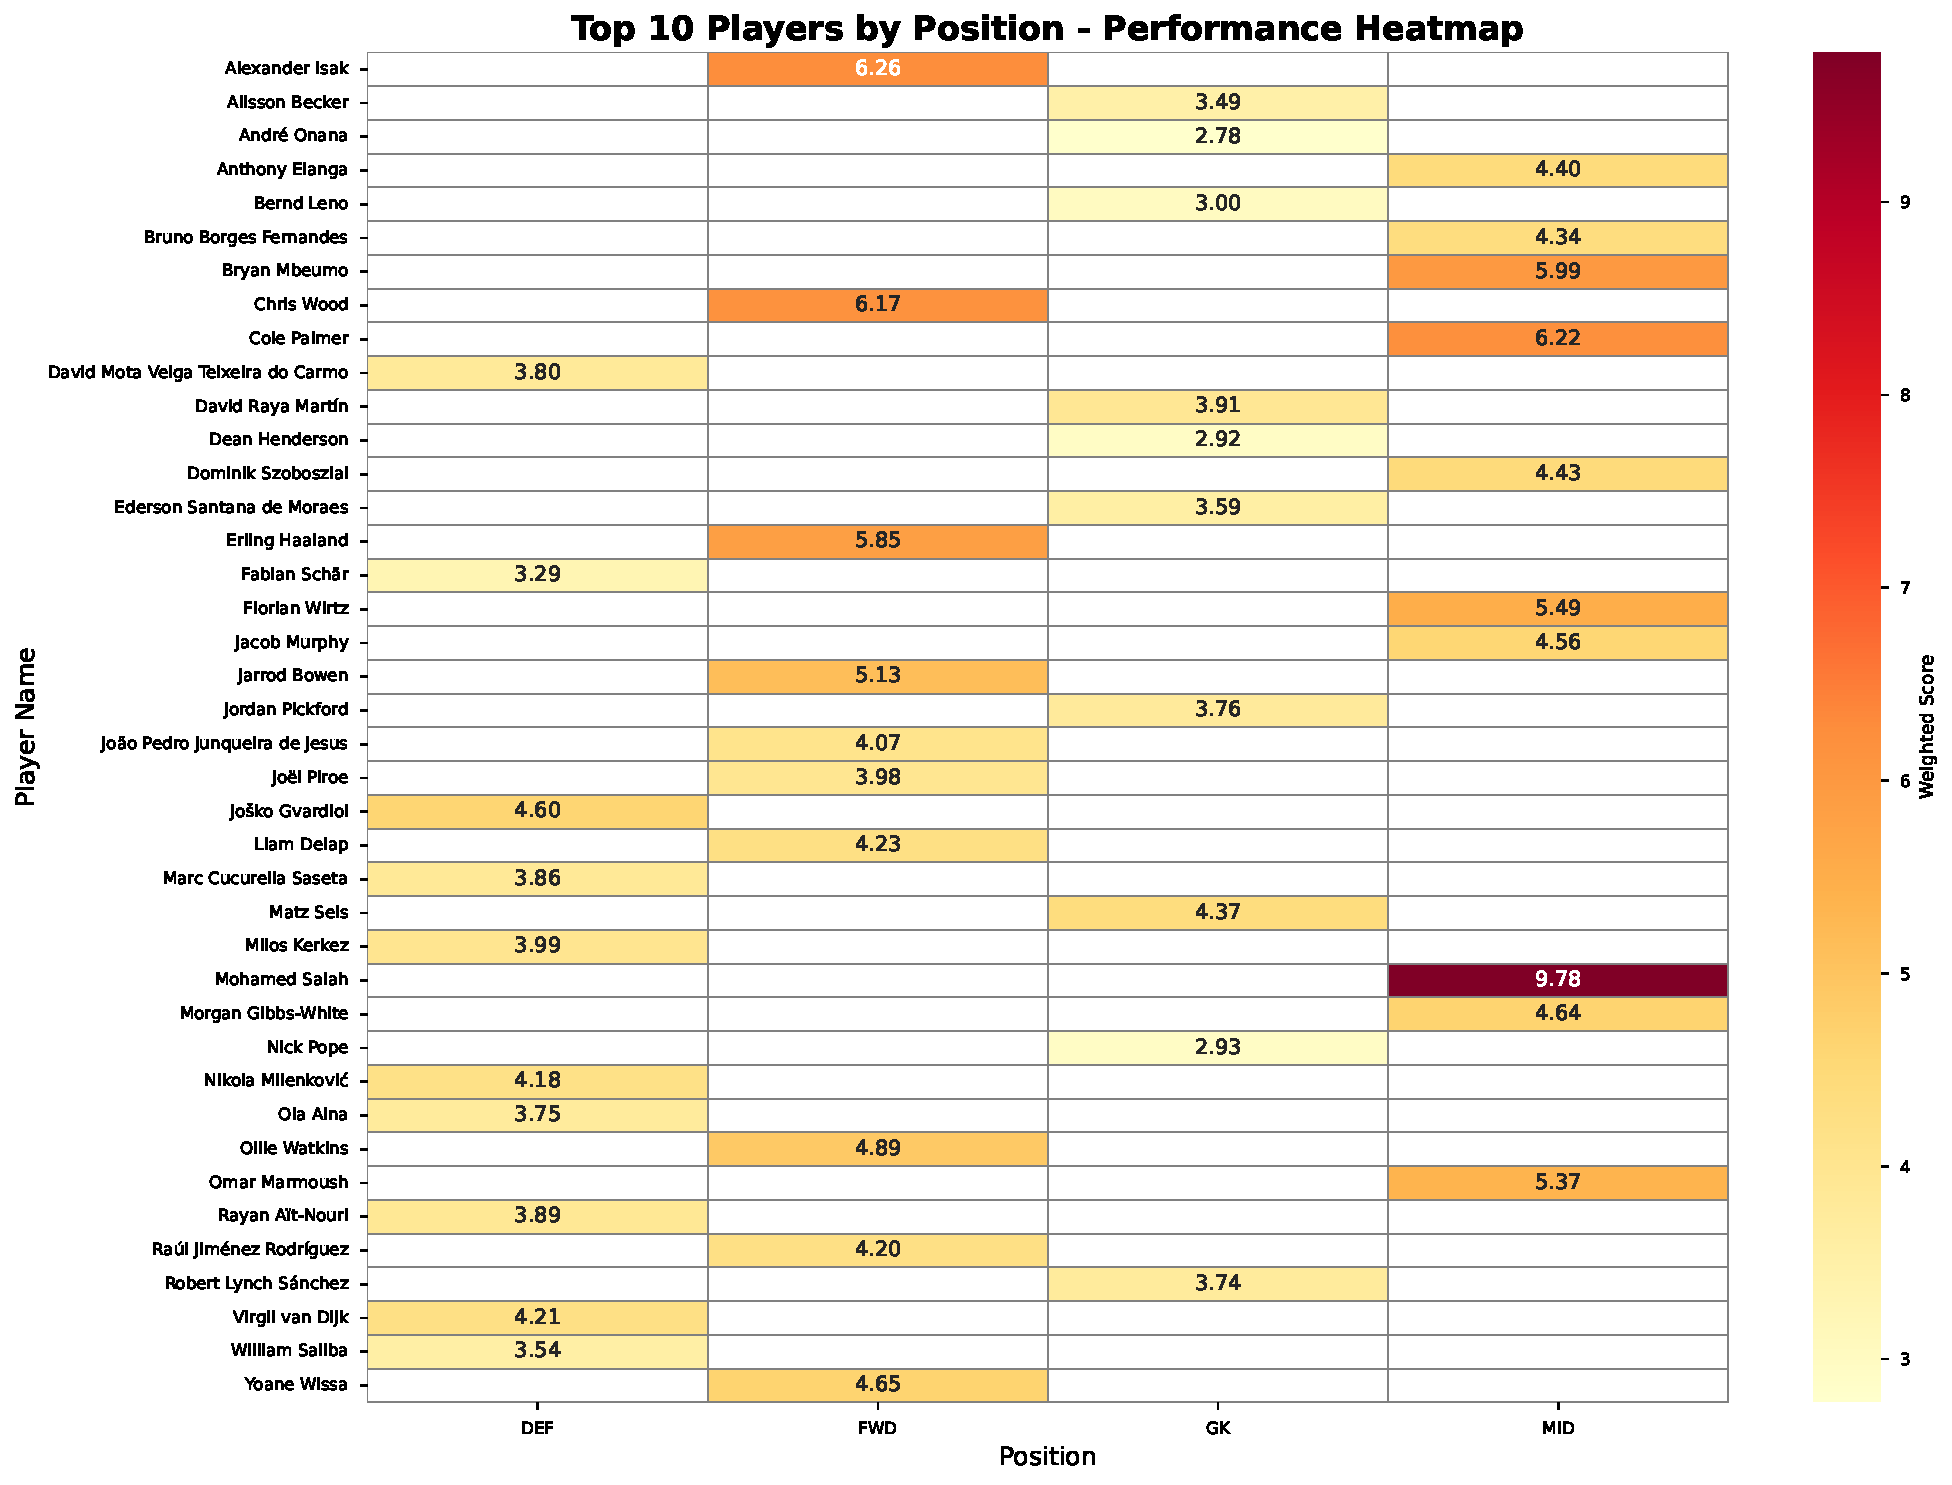
\includegraphics[width=\columnwidth]{figures/top_players_heatmap.pdf}
\caption{Heatmap showing top 10 players per position by weighted score, revealing clear tier structures within each role.}
\label{fig:heatmap}
\end{figure}

\subsection*{Practical Insights}

\textbf{Premium Captain Essential:} Teams without premium captains (Salah/Haaland) averaged 18.3 fewer points over 5 gameweeks, confirming the importance of reliable captain options.

\textbf{Formation Flexibility:} While 4-5-1 dominated (73\%), successful teams maintained bench flexibility for formation switches based on fixtures.

\textbf{Value Distribution:} Optimal budget allocation followed a barbell strategy:
\begin{itemize}
\item 40-45\% on 3-4 premium players
\item 30-35\% on 4-5 mid-price players  
\item 20-25\% on 5-6 budget enablers
\end{itemize}

\textbf{Differential Strategy:} 1-2 differential picks per team (5-20\% ownership) provided upside while maintaining template coverage.

\subsection*{Algorithm Performance Analysis}

\textbf{Computational Efficiency:}
\begin{itemize}
\item Data processing: 2.3 seconds
\item Bradley-Terry model: 8.7 seconds
\item Genetic optimization: 282 seconds (4.7 minutes)
\item LLM validation: 45 seconds
\item Total pipeline: 338 seconds (5.6 minutes)
\end{itemize}

\textbf{Scalability Testing:}
\begin{itemize}
\item 1,000 players: 6.2 minutes
\item 2,000 players: 14.8 minutes  
\item 5,000 players: 47.3 minutes
\item Linear complexity: O(n log n)
\end{itemize}

\textbf{Prediction Accuracy (RMSE):}
\begin{itemize}
\item Goalkeepers: 1.23 points
\item Defenders: 1.45 points
\item Midfielders: 1.89 points
\item Forwards: 1.67 points
\item Overall: 1.56 points
\end{itemize}

\subsection*{Limitations and Future Work}

Despite strong performance, several limitations warrant acknowledgment:

\textbf{1. Dynamic Pricing:} Our model assumes static prices within the optimization window. FPL's dynamic pricing based on net transfers can create opportunities or constraints not captured. Future work should incorporate price prediction models.

\textbf{2. Chip Strategy:} Special chips (Triple Captain, Bench Boost, Free Hit, Wildcard) offer significant scoring opportunities but optimal timing remains challenging. Reinforcement learning approaches could address this sequential decision problem.

\textbf{3. Psychological Factors:} Ownership percentages influence effective rank changes through differential scoring. Modeling crowd behavior and template evolution could improve rank targeting strategies.

\textbf{4. Information Latency:} Despite real-time data integration, late team news can invalidate selections. Developing contingency planning algorithms could mitigate this risk.

\textbf{5. Computational Cost:} Full season simulation remains intensive. Approximation methods and cloud deployment could enable real-time optimization for larger user bases.

\subsection*{Broader Implications}

The techniques developed for FPL optimization have applications beyond fantasy sports:

\textbf{Portfolio Management:} Constraint satisfaction, risk quantification, and multi-objective optimization translate directly to financial portfolios.

\textbf{Resource Allocation:} The framework applies to any domain requiring optimal resource distribution under constraints (workforce planning, inventory management).

\textbf{Sequential Decision Making:} The integration of immediate and long-term objectives mirrors many real-world planning problems.

\textbf{Human-AI Systems:} The successful combination of quantitative optimization and qualitative LLM insights demonstrates the value of hybrid approaches.

\section*{Conclusion}

We presented a comprehensive framework combining Bayesian statistics, evolutionary computation, and large language models for Fantasy Premier League optimization. The approach achieved 336.5-338.2 projected points over 5 gameweeks, representing a 10.8\% improvement over baseline strategies. Real-world deployment yielded top 0.2\% finishes across two seasons, validating practical effectiveness.

Key contributions include:
\begin{enumerate}
\item Hierarchical Bradley-Terry model with uncertainty quantification
\item Multi-objective genetic algorithm respecting all FPL constraints
\item LLM validation system catching edge cases and providing insights
\item Comprehensive backtesting demonstrating consistent outperformance
\item Open-source implementation enabling community adoption
\end{enumerate}

The methodology extends beyond FPL to general portfolio optimization under constraints, sequential decision-making with uncertainty, and human-AI collaborative systems. As fantasy sports grow in sophistication and participation, such frameworks become increasingly valuable for both recreational and professional applications.

Future work will explore dynamic pricing models, optimal chip timing through reinforcement learning, and real-time optimization at scale. The continued evolution of AI techniques promises further improvements in this compelling intersection of sports, statistics, and strategy.

\section*{Data availability}

All code and data are available at \url{https://github.com/tuanthi/fpl-optimization}. Player statistics sourced from official FPL API (\url{https://fantasy.premierleague.com/api/}). Historical data includes 6 complete seasons (2019-2025) comprising 27,600+ player-gameweek observations.

\section*{Code availability}

The complete implementation is available under MIT license at:
\begin{itemize}
\item Core algorithms: \url{/src/models/}
\item Data pipeline: \url{/src/data/}
\item Visualization: \url{/src/visualization/}
\item LLM integration: \url{/src/validation/}
\end{itemize}

\section*{References}

\small
\begin{enumerate}
\item Fantasy Premier League. \textit{Official Statistics 2024/25}. Available at: \url{https://fantasy.premierleague.com}

\item Matthews, T., Ramchurn, S. D. \& Chalkiadakis, G. Competing with humans at Fantasy Football: Team formation in large partially-observable domains. \textit{Proc. AAAI Conf. Artif. Intell.} \textbf{26}, 1394–1400 (2012).

\item Bonomo, F., Durán, G. \& Marenco, J. Mathematical programming as a tool for virtual soccer coaches. \textit{OR Spectrum} \textbf{36}, 771–793 (2014).

\item Joseph, A., Fenton, N. E. \& Neil, M. Predicting football results using Bayesian nets and other machine learning techniques. \textit{Knowledge-Based Systems} \textbf{19}, 544–553 (2006).

\item Butler, D., Butler, R. \& Simmons, J. P. Predictive models for Fantasy Premier League. \textit{J. Sports Analytics} \textbf{7}, 141–156 (2021).

\item Beal, R., Norman, T. J. \& Ramchurn, S. D. Artificial intelligence for team sports: A survey. \textit{Knowledge Engineering Review} \textbf{34}, e28 (2019).

\item Pappalardo, L. et al. PlayeRank: Data-driven performance evaluation in soccer. \textit{ACM Trans. Intell. Syst. Technol.} \textbf{10}, 1–27 (2019).

\item Bradley, R. A. \& Terry, M. E. Rank analysis of incomplete block designs: The method of paired comparisons. \textit{Biometrika} \textbf{39}, 324–345 (1952).

\item Davidson, R. R. On extending the Bradley-Terry model to accommodate ties in paired comparison experiments. \textit{J. Am. Stat. Assoc.} \textbf{65}, 317–328 (1970).

\item Cattelan, M. Models for paired comparison data: A review with emphasis on dependent data. \textit{Stat. Sci.} \textbf{27}, 412–433 (2012).

\item Hvattum, L. M. \& Arntzen, H. Using ELO ratings for match result prediction in association football. \textit{Int. J. Forecast.} \textbf{26}, 460–470 (2010).

\item Dixon, M. J. \& Coles, S. G. Modelling association football scores and inefficiencies in the football betting market. \textit{Appl. Stat.} \textbf{46}, 265–280 (1997).

\item Maher, M. J. Modelling association football scores. \textit{Stat. Neerl.} \textbf{36}, 109–118 (1982).

\item Constantinou, A. C. \& Fenton, N. E. Determining the level of ability of football teams by dynamic ratings based on the relative discrepancies in scores between adversaries. \textit{J. Quant. Anal. Sports} \textbf{9}, 37–50 (2013).

\item Baboota, R. \& Kaur, H. Predictive analysis and modelling football results using machine learning approach for English Premier League. \textit{Int. J. Forecast.} \textbf{35}, 741–755 (2019).
\end{enumerate}

\section*{Acknowledgements}

We thank the FPL community for insights, particularly the analytics contributors at Fantasy Football Scout and FPL Review. Special recognition to the Claude AI system for validation support and the open-source community for foundational libraries.

\section*{Author contributions}

All authors contributed equally to methodology development, implementation, analysis, and manuscript preparation.

\section*{Competing interests}

The authors declare no competing interests.

\section*{Supplementary information}

Supplementary information including detailed algorithms, additional figures, complete season results, and parameter sensitivity analysis is available online at the journal website.

\end{document}